\subsection{Queries} \label{sec:queries}
In order to verify the produced schedule and output relevant data, we have included several queries which can be run in \gls{smc}.
We want to verity that we do not fall below the battery threshold, and the payloads that are scheduled are actually executed.
Additionally, we want to monitor different variables in order to present the user with all the relevant data we are able to extract.\\
All probability queries are run with a confidence factor of $95\%$.

\subsubsection*{Verifying the Battery Capacity}
It is expected that battery usage in the \gls{smc} model differs from that in the \gls{cora} model as they use two different battery models, Ideal and \gls{kibam}.
The usage may also vary because of the possible differences in payload execution time.
The time it takes to complete one payload in \gls{cora} are constant but in \gls{smc} it may vary, as we want to model the uncertainty, which is done by using the time range that was defined by the user in the payload description.

We expect that we will use more energy in the \gls{smc} model because \gls{kibam} underestimates the energy consumption whereas the model used in \gls{cora} will overestimate.
The \gls{smc} model is also guaranteed to use less or equal amounts of time to complete a payload.
This is due to the \gls{cora} model using the worst case time when executing the payloads.
% impotant
\begin{equation} \label{eq:smca}
	Pr\; [<=ScheduleLength] \; (<>\; a\ <\ 0.1)
\end{equation}
Query \ref{eq:smca} will result in a probability that reflects the risk of the battery's available charge falling below $0.1$.
We added this query as depletion of the available charge can result in scheduled payloads being skipped.

\begin{equation} \label{eq:smcb}
	Pr\; [<=ScheduleLength] \; (<>\; b\ <\ ((1-c)*C) * (ThresholdPercentage\ /\ 100)
\end{equation}
Running query \ref{eq:smcb} results in the probability of the bound charge falling below the user specified threshold e.g. $40\%$ of the maximum battery capacity.
If this would occur, the nanosatellite would enter its safe mode.
The query has been included as falling below the threshold is considered a fail state.

\begin{equation} \label{eq:smctotal}
	Pr\; [<=ScheduleLength] \; (<>\; b\ +\ a\ <\ C\ *\ (ThresholdPercentage\ /\ 100)
\end{equation}
Query \ref{eq:smctotal} is the third and last query that may be used to ensure the battery capacity does not fall below the threshold.
This query indicates that the sum of available and bound charge may not fall below the specified threshold.

All of these queries are relevant to verify that the battery will not go below the threshold.
However, as it may take considerable time to run a probability query, as it is unpredictable how many simulations it will run, we have chosen to only include query \ref{eq:smctotal} in the tool.
This query is chosen above the others as it is ultimately the one describing the nanosatellite's \gls{soc}.

\subsubsection*{Verifying the Payload Order}
% impotant
The probability for the case were at least one of the scheduled payloads are skipped, is given by running the query \ref{eq:smc3}.
A payload may be skipped because one of its restrictions are not uphold, or because there is not enough power to execute it.
This query itself does not provide any information that can be used to identify what went wrong, but the user may inspect the results of the other queries in order to find the reason.
\begin{equation} \label{eq:smc3}
Pr\; [<=ScheduleLength] \; (<> \ skips \ !=\ 0)
\end{equation}

% extra
\begin{equation} \label{eq:smc4}
	simulate\ 100 \; [<=ScheduleLength] \; \{active, \; Processor.Running\}
\end{equation}
Query \ref{eq:smc4} is used in conjunction with query \ref{eq:smc3}.
This is just 100 simulations which respectively represent one random trace.
However in case any payloads were skipped during these simulations, it will be possible to find which was skipped at what time.\\
What \ref{eq:smc4} does, is indicating what payload is supposed to execute at what time, and whether or not it was.

As these queries support each other and query \ref{eq:smc4} is just a 100 simulation and therefore more predictable in the time it takes to complete, both will be included in the tool.

\begin{figure}[H]%
	\centering
	\subfloat
	{{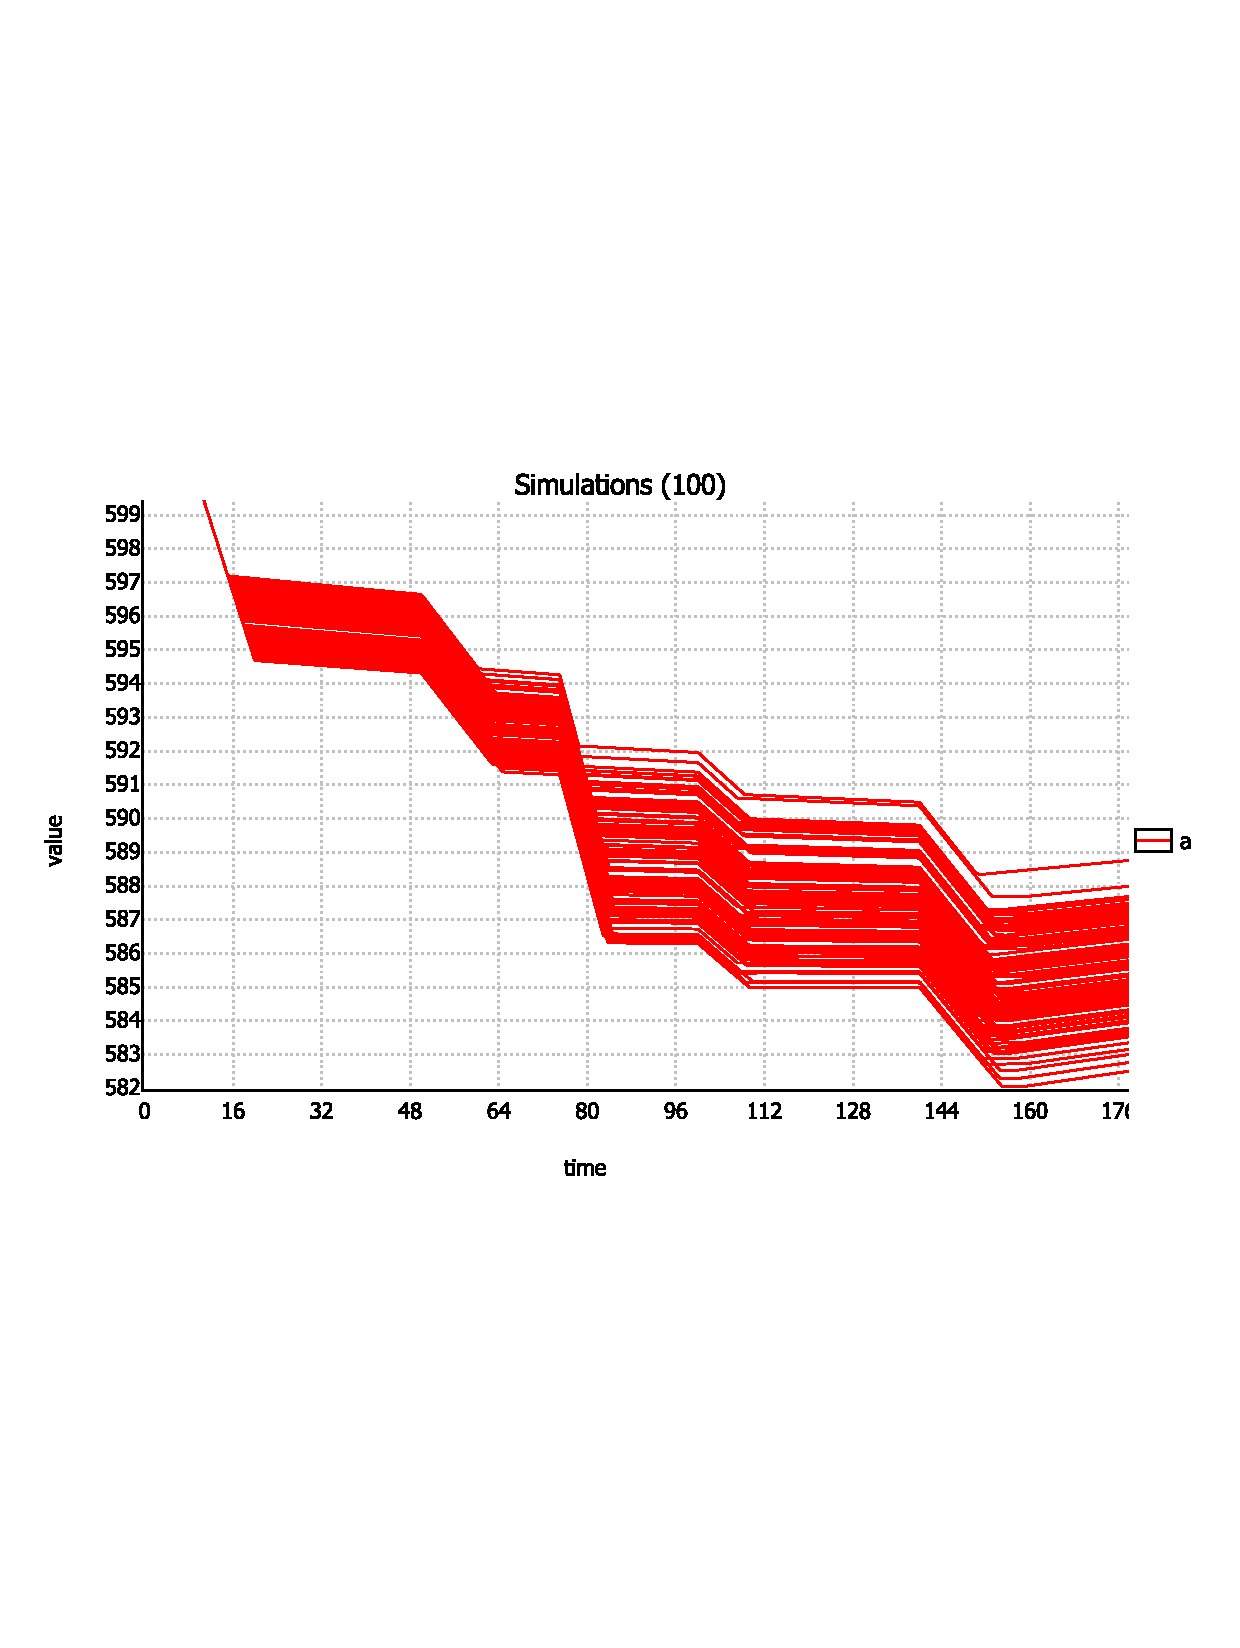
\includegraphics[width=7cm, trim={0 8cm 0 6cm},clip] {graphics/simulation_graphs/SimulationsA100.pdf} }}%
	\qquad
	\subfloat
	{{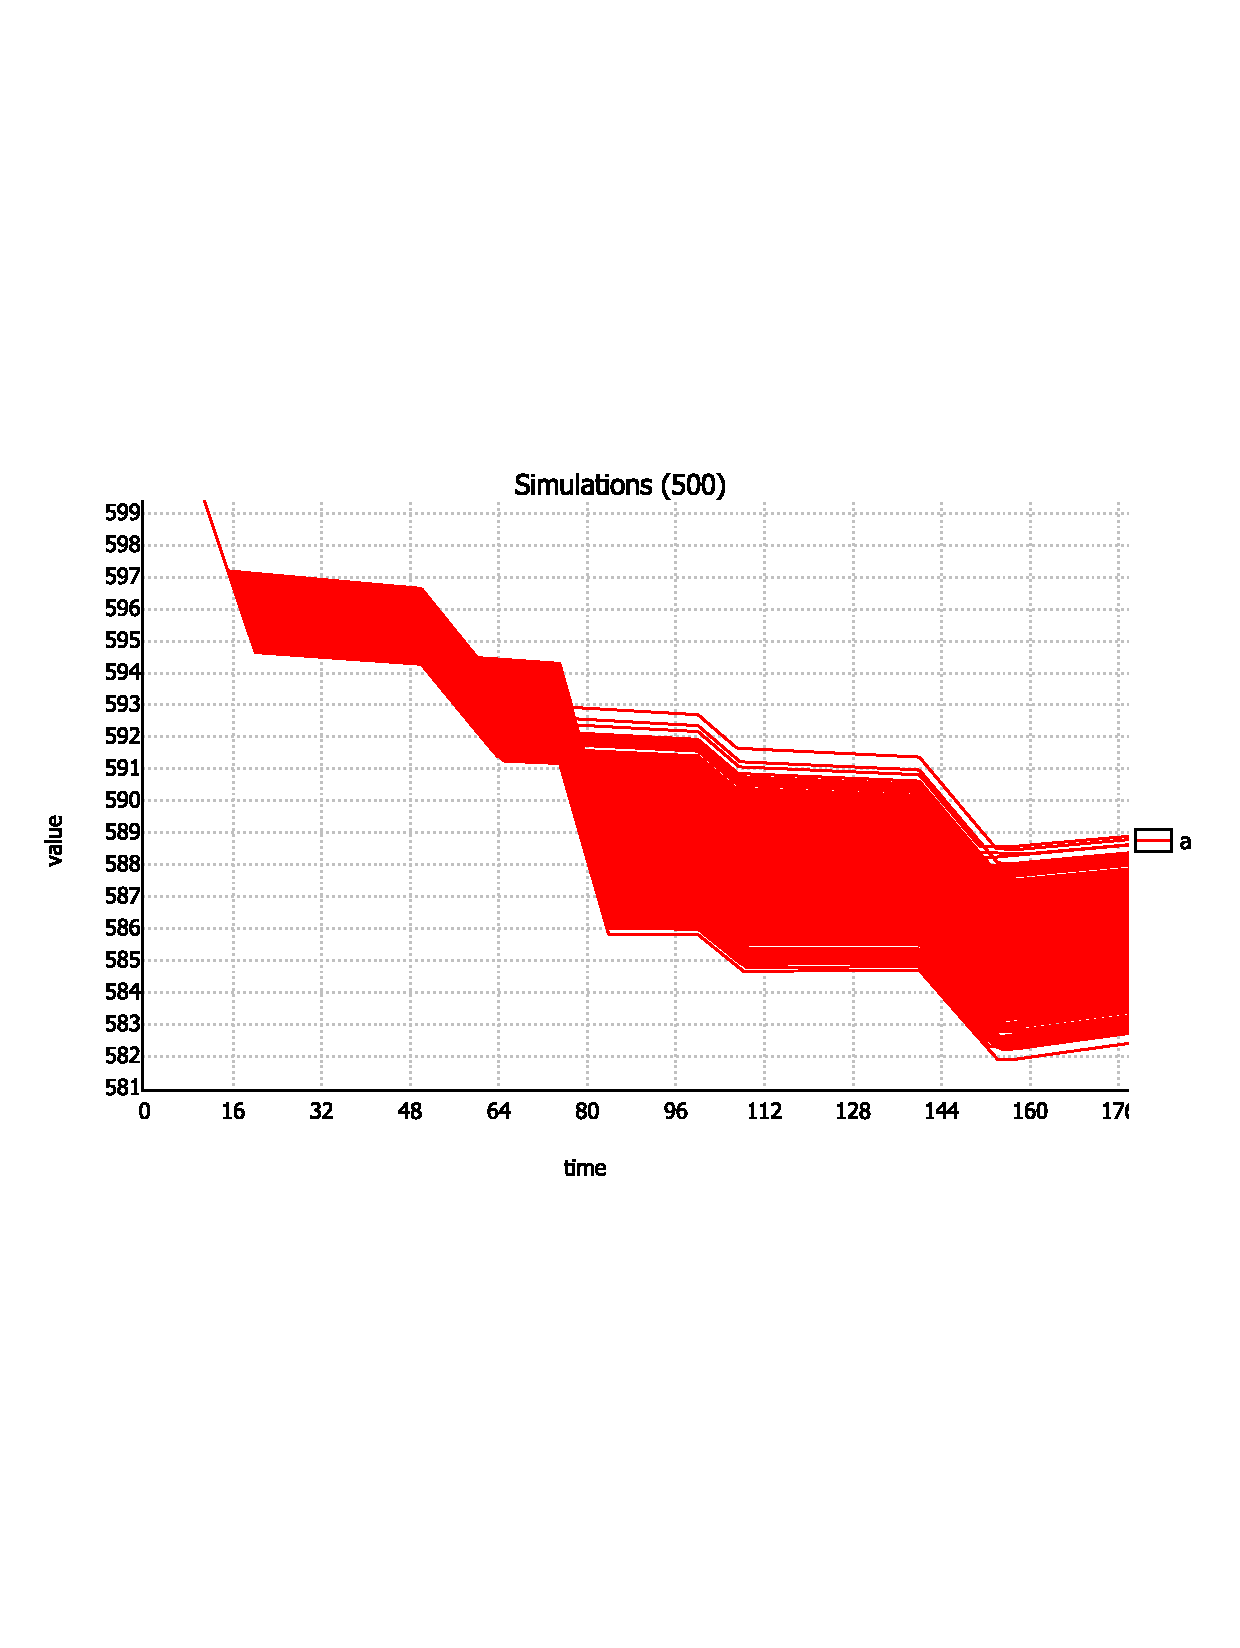
\includegraphics[width=7cm, trim={0 8cm 0 6cm},clip] {graphics/simulation_graphs/SimulationsA500.pdf} }}%
	\caption{100 simulations(left) versus 500 simulations(right) over available energy \uppVar{a} in \gls{smc}}%
	\label{fig:sim_amount}%
\end{figure}
In query \ref{eq:smc4} it is specified that we want to run the simulation 100 times, the reason for this is that we believe 100 simulations is adequate to give a reasonable representation of the values' ranges.
In \cref{fig:sim_amount} we see two graphs, one where the simulation have been run 100 times and one where it have been run 500 times.
The lowest observed value of \uppVar{a} is similar in both graphs, $182$ in the one with 100 simulations and $181.9$ in the one with 500 simulations.
The highest value observed by the end of the simulations were $188.8$ versus $189$.
In both cases the 500 simulations displays a wider range for the value, however the query running 100 simulations took 9 seconds, whereas the one with 500 took 55 seconds.\\
With the small differences to the final output and the large amount of time saved we conclude that running 100 simulations will give an acceptable range in short time.
Therefore we will use 100 simulations for all queries of the type simulation.
%It should also be noted that the simulations are run in order to provide indsight to the user, and should not be use

\subsubsection*{Other Information}
\begin{equation} \label{eq:smc5}
	simulate\ 100 \; [<=\ ScheduleLength]\; \{ a,\ b\}
\end{equation}
Query \ref{eq:smc5} provides two time series that reflects the two wells of the battery, \uppVar{a} and \uppVar{b}.
This is useful for the user as they might want to discard the schedule if it uses more energy than what they are comfortable with. Even if we do not go below the threshold, it may be to expensive to execute the schedule.

% extra
\begin{equation} \label{eq:smc6}
	E \; [<=\ ScheduleLength;\ 100]\; ( max:\ earnings)
\end{equation}
Query \ref{eq:smc6} finds the accumulated profit for the schedule.
We will not judge a schedule based on this value, we will let the user decide if it is acceptable.
However, the schedule is produced to maximise this value, see \myref{sec:cora}, and should therefore be viable.
The profit is an abstract variable and we will not be able tell whether or not it is satisfactory.

The three last queries, \ref{eq:smc4}, \ref{eq:smc5}, and \ref{eq:smc6}, are tested with simulations.
The simulations are great for giving the user insight in the behaviour of the nanosatellite when executing the schedule. \\
It does however not set any guarantees for the correctness or robustness of the schedule as it only displays the result of the path taken during each of the simulations.
